%!TEX root = main.tex
\chapter{Related Work}

In this chapter, we will cover the literature of the two main axes of research presented. First, an overview of the recent literature on photometric stereo is discussed. An emphasis is put on dealing with various illumination conditions, from controlled laboratory conditions to the harder case of outdoor lighting. Then, a review of prior art in lighting and camera calibration is presented. For the latter, we will mainly focus on horizon line estimation, which provides the main extrinsic parameters with respect to the earth.


\section{Photometric Stereo}


\begin{figure}
\centering
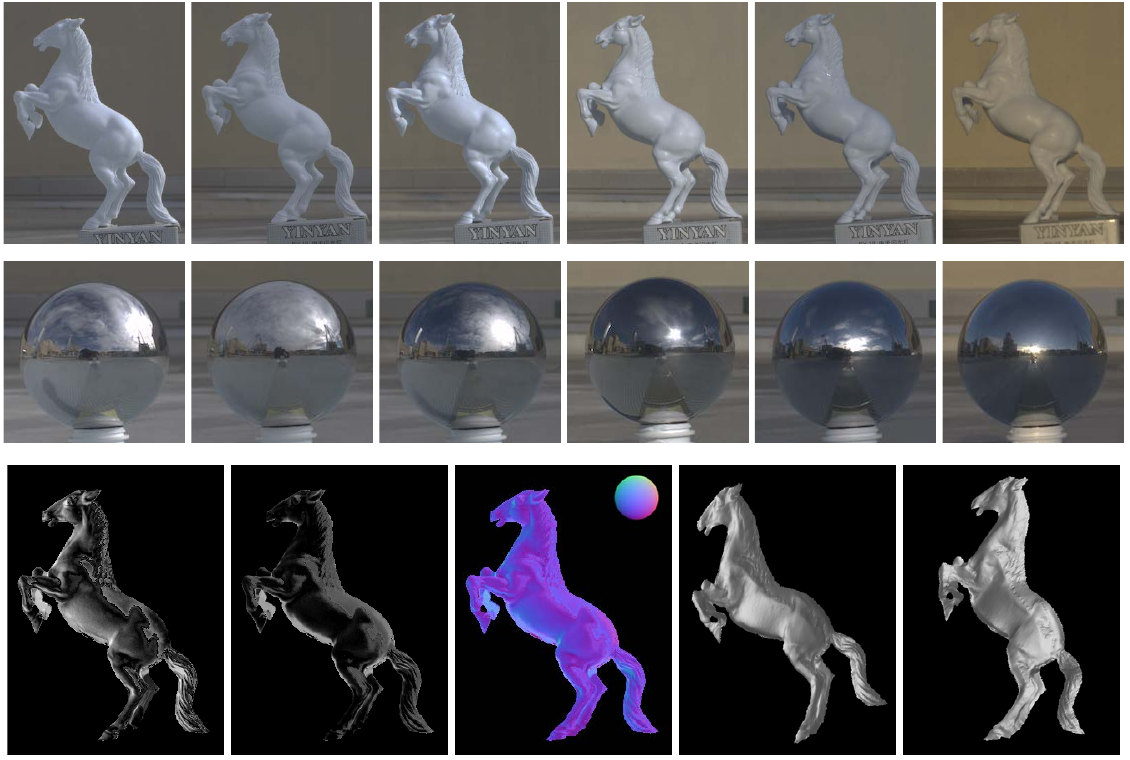
\includegraphics[width=0.96\linewidth]{3rdparty/yu-summary.png}
\caption[State-of-the-art calibrated photometric stereo]{When performing photometric stereo on images (top row), using a chrome sphere as light probe to capture the illumination (middle row) leads to a richer lighting model than the traditional point light source approach. Results are shown on the bottom row, showing the normal map $\mathbf{n}$ displayed as $\mathbf{n}\cdot\mathbf{l}$ with lighting $\mathbf{l}$ coming from $\left[-\nicefrac{1}{\sqrt{3}}, \nicefrac{1}{\sqrt{3}}, \nicefrac{1}{\sqrt{3}}\right]^T$ (first image) and $\left[-\nicefrac{1}{\sqrt{3}}, \nicefrac{1}{\sqrt{3}}, \nicefrac{1}{\sqrt{3}}\right]^T$ (second image). The third image shows the color-coded normal map. The fourth and fifth images show novel views of the reconstructed 3D surface. Figure taken from~\cite{yu-iccp-13}.}
\label{fig:yu_summary}
\end{figure}

As shown in Woodham's seminal work~\cite{woodham-opteng-80}, for Lambertian surfaces, calibrated PS computes a (scaled) normal vector in closed form as a simple linear function of the input image pixels; this linear mapping is only well-defined for images obtained under three or more (known) non-coplanar lighting directions. 
% intro on PS
Since its inception in the early 80s, it has been explored under many an angle. Whether it has been to improve its ability to deal with complex materials~\cite{alldrin-cvpr-08}, lighting conditions~\cite{alldrin-cvpr-08,basri-ijcv-07,johnson-cvpr-11,oxholm-eccv-12} or enhance other techniques like multiview stereo~\cite{snavely-ijcv-08}, the myriad of papers published on the topic are testament to the interest this technique has garnered in the community. A more detailed overview of general PS can be found in the recent, excellent review in~\cite{shi-tpami-18}. While most of the papers on this topic have focused on images captured in the lab, recent progress has allowed the application of PS on images captured outdoors, lit by the more challenging case of uncontrollable, natural illumination. 

% ask the question: how many images do we need?
A central question to any PS practitioner is that of the quality and amount of data required to achieve good performance. What should the lighting conditions be during data capture? How many images (illumination conditions) are needed? What is the shortest time interval required to collect these samples? 

In the lab, theoretical analyses for Lambertian surfaces, lit by point light sources, reveal that the minimum number of images is three~\cite{woodham-opteng-80} and that the optimal light configuration yields an orthogonal triplet of light directions~\cite{drbohlav-iccv-05}. While such theoretical guarantees are reassuring, they are however much harder to obtain for the case of more complex, non-Lambertian reflectance, or with more general lighting models. Thus, practitioners are left without guidance in the task of determining when to stop capturing data, an inherently tedious trial-and-error process. As a result, it is not rare for PS datasets to include hundreds of images~\cite{alldrin-cvpr-08} in an uncertain attempt to obtain accurate reconstruction. 

Subsequent work on outdoor PS has struggled to meet the light non-coplanarity requirement since, over the course of a day, the sun shines from directions that nearly lie on a plane. These co-planar sun directions then yield an ill-posed problem known as two-source PS; despite extensive research using integrability and smoothness constraints~\cite{onn-ijcv-90,hernandez-pami-11}, results still present strong regularization artifacts on surfaces that are not smooth everywhere. To avoid this problem in outdoor PS, authors initially proposed gathering months of data, watching the sun elevation change over the seasons~\cite{abrams-eccv-12,ackermann-cvpr-12}. More recently, Shen~{\em et al.}~\cite{shen-pg-14} noted that the coplanarity of the daily sun directions actually varies throughout the year, with single-day outdoor PS becoming more ill-posed at high latitudes near the winter solstice, and worldwide near the equinoxes. A creative solution to this problem was proposed in~\cite{hung-wacv-15}, but it is limited to objects that can be placed on a small moving platform. Therefore, capturing more data for fixed, large objects meant until recently waiting days, or even months, potentially~\cite{ackermann-cvpr-12,abrams-eccv-12}. 


% richer lighting models
To compensate for limited sun motion, other approaches use richer illumination models that account for additional atmospheric factors in the sky. One way to achieve this is by employing \mbox{(hemi-)spherical} environment maps~\cite{debevec-siggraph-98} of real sky captures~\cite{yu-iccp-13,shi-3dv-14,hung-wacv-15}. By inserting light probes into the scene, one is able to capture both the object appearance and its illumination at the same time. An example of one of those methods proposed by Yu et al.~\cite{yu-iccp-13} performing single-day photometric stereo is shown in fig.\ref{fig:yu_summary}. In their work, they propose an iterative method that performs two steps in alternation. First, they estimate the normal using standard photometric stereo. Then, this estimated normal defines a new visibility hemisphere, which in turn leads to a slightly different lighting. These two steps can be repeated until convergence, usually in 3-5 iterations. 

A second way to use richer illumination for photometric stereo is to synthesize the sky using a parametric sky model~\cite{inose-tcva-13,jung-cvpr-15}. This leads to a more constrained formulation of photometric stereo, enabling the relaxation of the calibration requirements. As such, semi-calibrated methods like the one proposed by Jung et al.\cite{jung-cvpr-15} began to appear. In their work, they don't need the capture of the full environment map through a light probe, removing the full calibration requirement. They propose to estimate the albedo of the surface using the first eigenvector of the observed pixels in RGB space. However, their technique is not fully uncalibrated, as they rely on the precise geolocation of the camera in order to constrain the sun path in the sky on a single axis. An example of the results obtained by this algorithm is shown in fig.~\ref{fig:jung_summary}.


% Using a large database of real sky images, Hold-Geoffroy~{et al.}~\cite{holdgeoffroy-iccp-15} showed that partly cloudy days are in fact better for single-day outdoor PS since clouds obscure and further scatter sun light, causing an out-of-plane shift in the effective direction of illumination. Subsequently~\cite{holdgeoffroy-3dv-15}, they also showed that good cloud coverage conditions for stable solutions may be observed in the sky within very short time intervals of just above one hour. 

%While capturing more data in the lab can be done relatively easily, the same cannot be said for outdoor imagery. Indeed, one does not control the sun and the other atmospheric elements in the sky; so one must wait for lighting conditions to change on their own. 

%Luckily, techniques that reduce the requirement to a single day's worth of data have also been proposed~\cite{yu-iccp-13,shen-pg-14,jung-cvpr-15}. However, this is still much longer than what can be done in the lab, where light sources can be waved around rapidly and data be captured in minutes. And although recent work has investigated which days provide more favorable atmospheric conditions for outdoor PS~\cite{shen-pg-14}, so far, no study has systematically demonstrated the performance of outdoor PS with less than a full day's worth of data.


% solar plane, nearly singular (ill-conditioned) light matrix, 2-image PS
% regularization breaks at (sharp) surface discontinuities

% webcams, solar plane


\begin{figure}
\centering
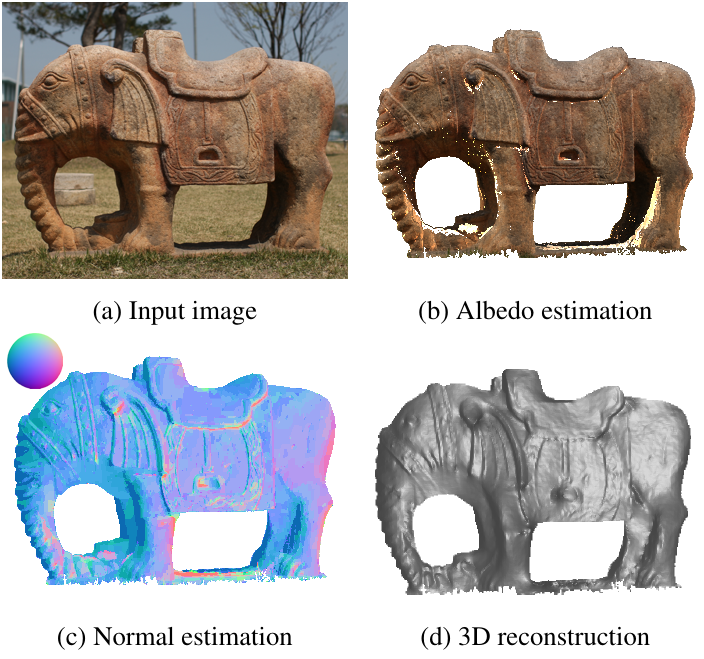
\includegraphics[width=0.50\linewidth]{3rdparty/jung-summary.png}
\caption[State-of-the-art semi-calibrated photometric stereo]{Example of single day outdoor photometric stereo without light probe inserted. Figure taken from~\cite{jung-cvpr-15}.}
\label{fig:jung_summary}
\end{figure}

Despite these developments, calibrated~\cite{yu-iccp-13} and semi-calibrated~\cite{jung-cvpr-15} (based on precise geolocation) outdoor PS are still prone to potentially long waits for ideal conditions to arise in the sky; and verifying the occurrence of such events is still a trial-and-error process.

So far, deep learning had only been applied for photometric stereo in indoor scenarios with rich and controlled illumination~\cite{yu-iccv-17,santo-iccv-17,taniai-arxiv-18,shi-tpami-18}, focusing on learning inverse functions for non-Lambertian reflectances.

%\cite{yu-iccv-17,santo-iccv-17,taniai-arxiv-18} Deep learning methods applied to photometric stereo (not one-day)

% Talk about DiLiGent~\cite{shi-tpami-18}? (Their objects have homogeneous material, with piecewise constant albedo, our method would work with any albedo pattern using the division trick. Also, only normal maps, no 3D models. Their sampling of 96 lighting directions does not approximate well the path of the sun through a day.)

% single image (nishino, deep learning)
Finally, under more extreme ambiguity, techniques for shape-from-shading (SfS)~\cite{Horn1989,Zhang1999,Langer1994,oxholm-eccv-12,johnson-cvpr-11,barron-pami-15} attempt to recover 3D normals from a single input image, in which case the shading cue alone is obviously insufficient to uniquely define a solution. Thus, SfS relies strongly on priors of different complexities and deep learning is quickly bringing advances to the field~\cite{eigen-iccv-15,shu-cvpr-17,wu-nips-17,shu-cvpr-17}.


\section{Models for approximating outdoor lighting}

Lighting is the fundamental element that makes up all images. As Paul Cézanne said, ``there is no model; there is only color.'' Knowing the lighting of a scene allows for a deeper understanding of the camera, the scene and its materials, and enables a myriad of applications like automatic virtual object insertion.

In this section, we will present the most notable physically-based and analytical outdoor illumination models as well as the methods used to estimate their parameters from images.

\subsection{Physically-based outdoor illumination models}

Physically-based models seek to generate accurate representations of the sky. They are based on physical simulations to provide the luminance distribution of the sky in function of the sun position and some atmospheric characteristics. They are usually slow to evaluate, but typically closer to real sky luminance measurements than analytical models.

The first model to explain the main physical phenomenons coming into play to form daylight was published by Nishita et al. in their seminal work of 1993~\cite{nishita1993display}. The most important physical phenomenon models interactions of the electromagnetic field (visible light, in this case) with small aerosols. Specifically, it encompasses interactions with particles having a radius $r$ significantly smaller than the light wavelength $\lambda$. This domain of interactions, characterized by $\frac{2\pi r}{\lambda} \ll 1$, is called the Rayleigh scattering and predicts the behavior of light when it interacts with nitrogen and oxygen, the major constituents of air. According to this theory, the amount of scattering happening in the atmosphere decreases proportionally to $\lambda^4$. In the visible spectrum, this translates in small wavelengths (blues) being much more scattered than large wavelengths (reds), explaining why the sky is perceived blue by the human eye.

The second most important type of interactions solves Maxwell's equations for the case of particles with a radius $r$ roughly the same size as the light wavelength $\lambda$. This regime ($\frac{2\pi r}{\lambda} \approx 1$) represents interactions of light with heavier molecules like water particles in suspension in the atmosphere, in clouds or during fog. This domain of interactions is called Mie scattering and is responsible for the white appearance of the clouds.

Summing both Rayleigh and Mie scattering together gives luminance estimations very close to measurements performed during daylight, confirming the dominance of those two phenomenons for the appearance of the sky. Example of those simulations of those phenomenons are shown in fig.~\ref{fig:physics_simulations}.

\begin{figure}
\centering
\newcommand\Tstrut{\rule{0pt}{1\normalbaselineskip}}         % = `top' strut
\newcommand\Bstrut{\rule[-1.5em]{0pt}{0pt}}   % = `bottom' strut
\begin{tabular}{|c|c|}
\hline
\Tstrut Rayleigh Scattering & Mie Scattering \\ \hline
\rule{0pt}{5\normalbaselineskip}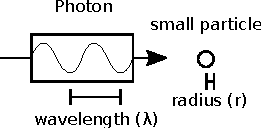
\includegraphics[width=0.25\linewidth]{simulation/small_particle.pdf} &
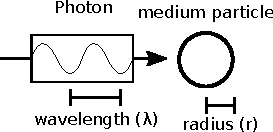
\includegraphics[width=0.25\linewidth]{simulation/medium_particle.pdf}\\
\rule{0pt}{1.5\normalbaselineskip}\Bstrut $\frac{2\pi r}{\lambda} \ll 1$ & $\frac{2\pi r}{\lambda} \approx 1$\\ \hline

\includegraphics[width=0.25\linewidth]{simulation/skydome_rayleigh.png} &
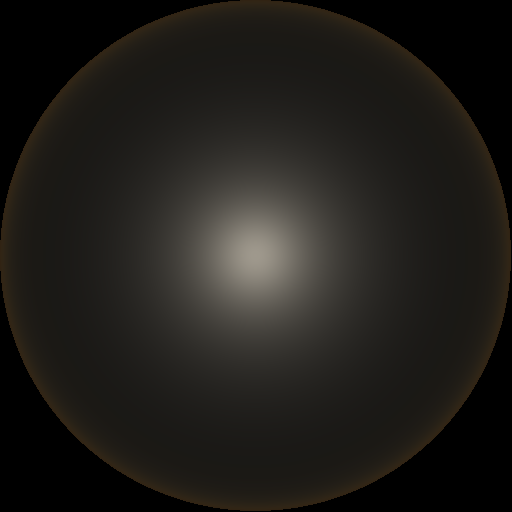
\includegraphics[width=0.25\linewidth]{simulation/skydome_mie.png} \\ \hline
\multicolumn{2}{|c|}{
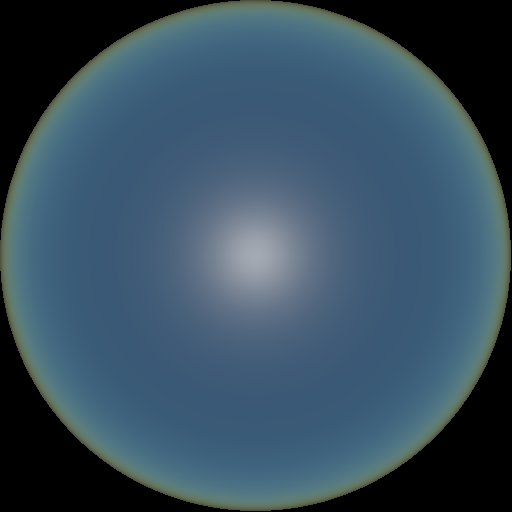
\includegraphics[width=0.25\linewidth]{simulation/skydome.png}} \\ \hline
\end{tabular}
\caption[Visualisations of the Rayleigh and Mie scattering]{Rayleigh (left) and Mie (right) scattering when the sun is at zenith. The images of the sky use the skyangular representation, where the zenith is at the center of the image and the horizon lies on the largest circle of the image. This representation is equivalent to a picture taken with a $180\degr$ fisheye lens pointed up at the sky.}
\label{fig:physics_simulations}
\end{figure}

In subsequent work, Nishita et al.~\cite{nishita1996display} enhanced their model by adding two elements: 1) the influence of ground albedo on the sky and 2) multiple scattering. A single scattering event per observed light ray was considered in the first formulation of their work. In this work, they consider multiple scattering interactions before observation.

Most published physically-based models are variants of the Rayleigh and Mie scattering, either with single or multiple scattering, as proposed in~\cite{nishita1993display,nishita1996display}, usually focusing on speeding up the simulation~\cite{oneal2005accurate}, slightly increasing agreement with measures of the real sky~\cite{haber2005physically,bruneton2008precomputed} or extending it to arbitrary atmospheres like oceans~\cite{elek2010real}.

Daylight is not the only phenomenon that received attention in the literature. A night sky model has also been developed~\cite{jensen2001nightskymodel}, taking into consideration the sun's reflection on the moon as well as the light emitted from the stars.

\subsection{Analytical outdoor illumination models}

Contrarily to physically-based models, analytical sky models are composed of a single empirically-derived closed-form equation to obtain the luminance of the sky. While they are typically used for rendering and for real-time applications because of their high evaluation speed, their accuracy is somewhat worse than physically-based models, giving skies that agree less with real skies measurements.

The first weather condition that was modeled in the literature is the overcast sky. Kimball and Hand~\cite{kimball1921sky} were the firsts to report in 1921 that cloudy days had higher luminosity near their zenith, and decreasing luminosity toward the horizon. Two decades later, Moon and Spencer~\cite{moon1942illumination} formulated the first luminance distribution model for the overcast sky. This work has been revisited and adopted as the CIE overcast sky model in 1996~\cite{cie1996s}. In this model, the luminance of the sky $Y_z$ in function of the zenith angle of a sky element $\theta$ is defined as
\begin{equation}
Y_z = \frac{1 + 2 \; \cos\left( \theta \right)}{3} \quad.
\end{equation}
To summarize, the sky luminance of overcast days is proportional to the $\cos$ of the zenith angle. While this model predicts quite accurately overcast days, it does not tell the whole story about daylight in general.

% The physical simulation of both Rayleigh and Mie scattering was also used as reference when developing the Preetham~\cite{preetham-siggraph-99} and Ho\v{s}ek-Wilkie~\cite{hosek-siggraph-12} analytical models. The parameters of those two analytic models were fit to the physical simulations using either a least square quadratic optimization or a spline, respectively.


\begin{figure}
\centering
\begin{tabular}{@{}c@{}c@{}c@{}c@{}}

\includegraphics[width=0.23\linewidth]{3rdparty/hw-004.jpg} &

\includegraphics[width=0.23\linewidth]{3rdparty/hw-005.jpg} &

\includegraphics[width=0.23\linewidth]{3rdparty/hw-006.jpg} &

\includegraphics[width=0.23\linewidth]{3rdparty/hw-007.jpg} \\
$T$ = 2 & $T$ = 4 & $T$ = 6 & $T$ = 8 \\
\end{tabular}
\caption[Examples of skies produced by the Ho\v{s}ek-Wilkie sky model]{Examples of skies produced by the Ho\v{s}ek-Wilkie sky model for various turbidity $T$ values. Figure from~\cite{hosek-siggraph-12}.}
\label{fig:hw_sky_model}
\end{figure}


For more general, non-overcast skies, Kittler~\cite{kittler1985luminance} was the first to propose a luminance distribution measurement strategy and predictive model, which eventually became the CIE standard sky model~\cite{darula-cie-sky}. Based on this model, Perez et al.~\cite{perez1993allweather} proposed a generalization called the all-weather sky luminance distribution model. This model defines the luminance of the sky dome as a function of the zenith angle of the considered sky element $\theta$ and the angular distance between this sky element and the sun position $\gamma$:
\begin{equation}
Y_z = \underbrace{\left( 1 + A e^{\nicefrac{B}{\cos\theta}} \right)}_{\text{geometric factor}} \cdot \underbrace{\left( 1 + C e^{D\gamma} + E \cos^2 \gamma \right)}_{\text{indicatrix function}} \;.
\label{eq:perez}
\end{equation}
This equation is parameterized by five coefficients ($A$-$E$) that can be varied to generate a wide range of skies. The first term in parenthesis represents the luminance decrease as the zenith angle increase while the second term is called an \emph{indicatrix function} and approximates the weather.


\begin{figure}
\centering
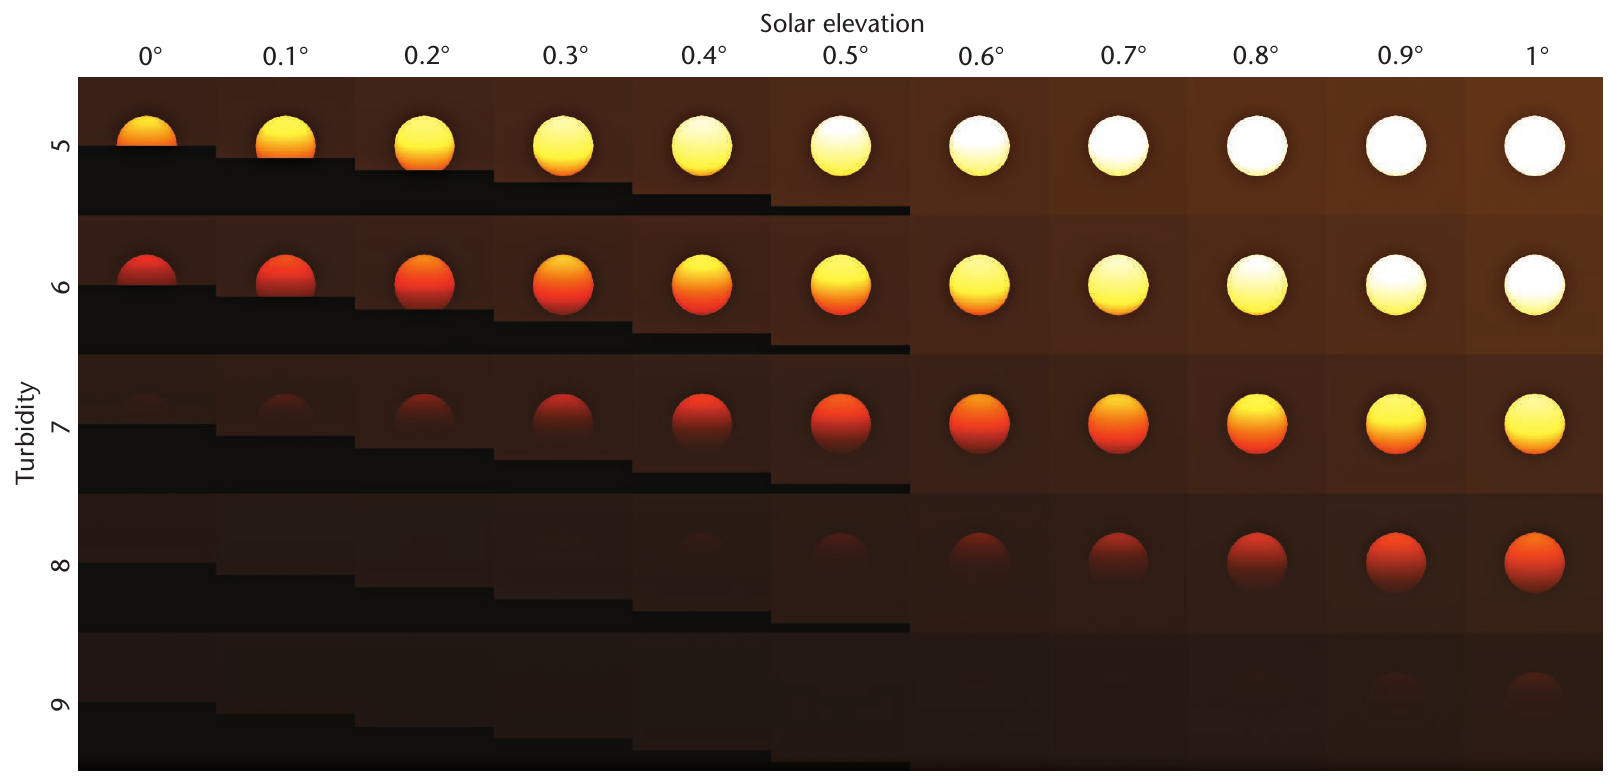
\includegraphics[width=0.96\linewidth]{3rdparty/hwsun-suns.png}
\caption[Examples of suns produced by the Ho\v{s}ek-Wilkie solar model]{Examples of suns produced by the Ho\v{s}ek-Wilkie solar model for various sun elevations and turbidity $T$ values. Figure from~\cite{hosek-siggraph-12}.}
\label{fig:hw_sun_model}
\end{figure}

Preetham et al.~\cite{preetham-siggraph-99} proposed to reduce the number of coefficients from five down to a single physically meaningful value: Linke's turbidity~\cite{mccartney1976optics}. This parameter is defined as
\begin{equation}
T = \frac{t_m + t_h}{t_m} \;,
\end{equation}
where $t_m$ is the optical thickness of the molecular atmosphere (devoid of haze), and $t_h$ is the optical thickness of the haze atmosphere. In order to apply this turbidity parameter to the Perez model, they perform the physical simulation proposed in~\cite{nishita1996display} by varying the turbidity $T$ between 2 and 6. They then fit the 5 parameters ($A$-$E$) of Perez's model to the simulation results using a Levenberg-Marquardt non-linear least squares optimization. They then obtain a linear function that maps the parameters optimization to the turbidity $T$. They also extend their model with chrominance, leading to the first analytical model with color. 
Eight years after this Preetham model was proposed, a critic was published~\cite{zotti2007critical} relating the relatively small valid turbidity range, the antisolar region being systematically too bright and the too smooth intensity peak toward the sun.

Lalonde and Matthews~\cite{lalonde-3dv-14} contributed to solving the lack of peakiness issue of the Preetham model by combining it with a novel empirical sun model. Ho\v{s}ek and Wilkie also proposed a sky luminance model~\cite{hosek-siggraph-12} that fixed most of the antisolar region mismatch while keeping the same turbidity $T$ parameter. In order to do so, they performed more simulations, still based on~\cite{nishita1996display}, and added 4 parameters to the indicatrix term of eq.~\eqref{eq:perez}. During their simulation, they sample the wavelength over eleven spectral channels from 320nm to 720nm, leading to an hyperspectral model that can be interpolated over the whole visible spectrum and slightly into the ultraviolet spectrum. Furthermore, they noted that the linear interpolation used by the Preetham model cannot account for abrupt variations at low solar elevations. To remedy this, they use a quintic-order Bezier polynomial to perform the fit between turbidity, wavelength, ground albedo and the 9 parameters ($A$-$I$) of their proposed analytical equation. An example of the sky dome produced by this sky model is shown in fig.~\ref{fig:hw_sky_model}. In subsequent work, they extended their model to include a solar radiance function~\cite{hosek-cga-13}, as shown in fig.~\ref{fig:hw_sun_model}. Some of the rendering capabilities of this model is shown in fig.~\ref{fig:hw_renders_model}. Finally, they added earth-like extrasolar skies capabilities to their model~\cite{wilkie2013predicting}.



\begin{figure}
\centering
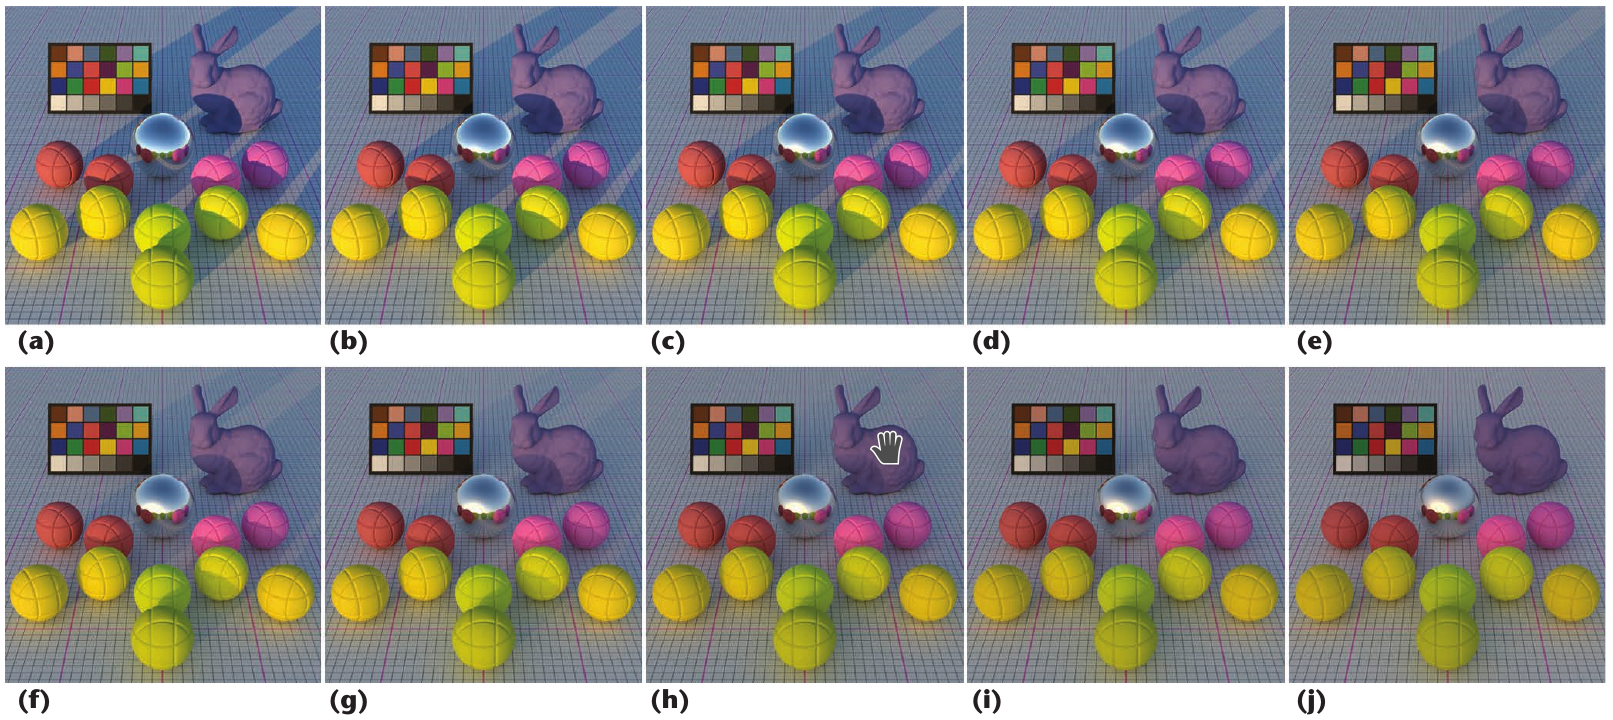
\includegraphics[width=0.96\linewidth]{3rdparty/hwsun-renders.png}
\caption[Examples renders lit by the Ho\v{s}ek-Wilkie solar and sky models]{Examples of renders lit by the Ho\v{s}ek-Wilkie solar and sky models. A sun elevation of $8\degr$ was used to produce these renders, with turbidities of (a) 1, (b) 2, (c) 3, (d) 4, (e) 5, (f) 6, (g) 7, (h) 8, (i) 9, and (j) 10. Images are tone-mapped to appear roughly equally bright. Figure from~\cite{hosek-siggraph-12}.}
\label{fig:hw_renders_model}
\end{figure}

\section{Parameters estimation for outdoor illumination models}

Aside from the fully overcast sky model, all sky models require some parameters to be estimated in order to reproduce a given sky. A fundamental parameter common to all non-overcast daylight sky models is the position of the sun in the sky. Most models then add some atmospheric parameters like turbidity to increase agreement between prediction and real sky measurements. The calibration of sky models consists into finding the sun position and some atmospheric properties. 

Those parameters change the appearance of the whole sky. However, when a camera takes a picture, the whole sky is usually not present in the image; typically, either a small region or no sky at all is visible. The following relates some techniques that perform the calibration of sky models from the limited view of a camera. 

Lalonde et al.~\cite{lalonde-ijcv-12} combine multiple cues, including shadows, shading of vertical surfaces, and sky appearance to predict the direction and visibility of the sun. This is combined with an estimation of sky illumination (represented by the Perez model~\cite{perez1993allweather}) from sky pixels~\cite{lalonde-ijcv-10}. 

Other techniques for single image illumination estimation rely on known geometry and/or strong priors on scene reflectance, geometry and illumination~\cite{barron-pami-15,barron2013rgbd,lombardi2016reflectance}. These priors are usually crafted for specific scenes, and typically do not generalize to large-scale outdoor scenes. Karsch et al.~\cite{karsch2014automatic} retrieve panoramas (from the SUN360 panorama dataset~\cite{xiao-cvpr-12}) with features similar to the input image, and refine the retrieved panoramas to compute the illumination. However, the matching metric is based on image content which may not be directly linked with illumination. 

Another class of techniques simplify the problem by estimating illumination from image collections. Multi-view image collections have been used to reconstruct geometry, which is used to recover outdoor illumination~\cite{haber2009relighting,lalonde-3dv-14,shan2015visual,duchene2015multiview}, sun direction~\cite{wehrwein2015shadows}, or place and time of capture~\cite{hauagge2014outdoor}. Appearance changes have also been used to recover colorimetric variations of outdoor sun-sky illumination~\cite{sunkavalli2008color}. 

% \subsection{Inverse graphics/vision problems in deep learning}

% \todo{enlever?}

% Following the remarkable success of deep learning-based methods on high-level recognition problems, these approaches are now being increasingly used to solve inverse graphics problems~\cite{kulkarni15dcign}. In the context of understanding scene appearance, previous work has leveraged deep learning to estimate depth and surface normals~\cite{eigen-iccv-15,bansal2016marr}, recognize materials~\cite{bell2015minc}, decompose intrinsic images~\cite{zhou2015intrinsic}, recover reflectance maps~\cite{rematas-cvpr-16}, and estimate, in a setup similar to physics-based techniques~\cite{lombardi2016reflectance}, lighting from objects of specular materials~\cite{georgoulis2016delight}. We believe ours is the first attempt at using deep learning for full HDR outdoor lighting estimation from a single image.


% \section{Camera calibration}

% \todo{faire comme PS}

% Geometric camera calibration is a widely studied topic that has a significant impact on a variety of applications including metrology~\cite{Criminisi2000}, 3D inference~\cite{Criminisi00,Fouhey2013} and augmented reality, both indoor~\cite{hedau-iccv-09,izadinia-cvpr-17} and outdoor~\cite{hoiem-cvpr-06}. As such, many techniques were developed to perform precise geometric calibration using a calibration target inserted beforehand in the image~\cite{Sturm1999,Zhang2002,Heikkila1997,Chen2004}. For after-the-fact calibration, most work on camera calibration aim to detect specific geometric objects in the image typically present in human-made environments~\cite{Rother2000,Melo2013}. Similarly, PoseNet~\cite{kendall-iccv-15} performs camera relocalization by jointly learning location and orientation. More recently, methods for straighting up photographs like Upright~\cite{Lee2014} recover calibration by finding vanishing points. Other work proposed to take advantage of lighting cues to calibrate~\cite{lalonde-ijcv-10,Workman2014}, circumventing the need for human-made environments. However, these techniques often fail on complex scenes where semantic reasoning is required to discard misleading textures and visual cues. To solve the need for high-level reasoning, deep convolutional neural networks were recently used to estimate field of view~\cite{Workman2015a} and horizon lines~\cite{Workman2016}, bringing camera calibration on single images to a wider variety of scenes.

% Understanding the limits of the human visual system has also received significant attention, with studies quantifying color sensitivity~\cite{fairchild2013color}, how reliably we can detect photo manipulations artifacts~\cite{Farid2010} and how people perceive distortion in street-level image-based rendering~\cite{Vangorp2013}. More recently, perceptual studies were performed to assess human appreciation on tasks like super-resolution~\cite{ledig-cvpr-17}, image caption generation~\cite{vinyals-cvpr-15} and video temporal alignment~\cite{papazoglou-accv-16}. 

